\section*{Instructions}
You will have \textbf{90} minutes to write code that should pass all
15 provided tests. \\
File in which all test are written is called \textbf{functions.test.js}.\\
The code for test is hashed, so You will not understand it’s details.\\

\begin{large}

  All tasks have to be implemented in this ONE and ONE ONLY file
  explicitly named \textbf{functions.js}. Any other name of file will
  not be accepted by automated checking server.

  After You will finish Yours implementation the
  \textbf{functions.js} have to be archived into the explicitly named
  \textbf{functions.zip} file, and this zip file have to be send onto
  the assignment.
  I do not accept any WORD or PDF or any other name or format.\\
  You have to create a file called \textbf{functions.js} and in this
  file create and export all functions/classes that are need by the
  tests, in given term:
\end{large}
\\
\begin{lstlisting}[language=json,firstnumber=1]
module.exports = {}
module.exports.example = example
\end{lstlisting}
Both of those files have to be inside same folder, Jest and NPM force this.\\
\newpage
\section*{How to create env for testing}
All information was shown on laboratory.
\begin{enumerate}
  \item Create new empty folder,
  \item Download archive with \textbf{\textit{functions.test.js}} file from \textbf{MS
    Teams Assignment},
  \item Install library
    \textbf{\textit{\href{https://jestjs.io/docs/getting-started}{JEST}}}
    \begin{enumerate}
      \item Open terminal/command-prompt and go into prviously
        created empty folder, call \\ \textbf{npm install --save-dev jest}
      \item in \textit{package.json} add: \\
\begin{lstlisting}[language=json,firstnumber=1]
"scripts": {
"test": "jest"
}
\end{lstlisting}
    \end{enumerate}
  \item To check if env was properly configured run: \\ \textbf{npm run test}
\end{enumerate}
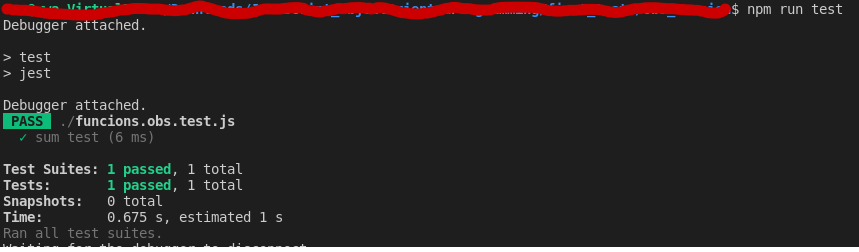
\includegraphics[width=\textwidth]{npm_run_test}
